\documentclass[12pt]{article}
\usepackage{Geoff,graphicx}

\title{Meeting notes 28-9-2017: Graph Matching}
\author{Geoff Iyer}
\date{}

\begin{document}
\maketitle

\section*{Quick Summary}

Using graph match, we can come up with some kind of feature comparison
algorithm.  I'm not sure what to call it. It's not exactly change detection but
it's similar.  Here is a rough overview. Given coregistered datasets $X,Y$ (so
$x_i$ corresponds to $y_i$), we do a graph match to get a second registration
$\rho: X\to Y$. We then compare the different registrations. Specifically, look
at the matches $x_i \to y_{\rho(i)}$ where the calculated match weight is
strong. Then for those particular $i$, compare $x_i$ to $ x_{\rho^{-1}}(i)$ and
$y_i$ to $y_{\rho(i)}$. In other words, look for points where the graphs match
well, but it does not agree with the actual coregistration. See examples at the end.

\section*{Problem Statement and Background Theory}

First we recall the problem statement. Let $G = (X,W_X)$, $H = (Y,W_Y)$ be
undirected, weighted graphs. Here $X, Y$ represent the nodes of $G, H$
(respectively), and $W_X,W_Y$ are the corresponding matrix of edge weights. For
convenience of notation we will assume $\abs{X} = \abs{Y} = N$. The extension to
the general case is quite straightforward. The goal of the Weighted Graph
Matching Problem (WGMP) is to find a bijection $\rho:X \to Y$ that minimizes the
squared difference of edge weights. Phrased in terms of matrices, our
minimization problem becomes
\begin{align}
  \label{eqn:WGMPperm} \text{argmin}_{P\text{ a permutation
  matrix}}\norm{PW_XP^T - W_Y}^2_F.
\end{align}
This problem is NP-hard, so we relax and look for an orthogal matrix.
\begin{align}
  \label{eqn:WGMPorthog} Q^* = \text{argmin}_{QQ^T=I}\norm{QW_XQ^T - W_Y}^2_F.
\end{align}
This problem is solved via eigenvectors of the graph laplacian.  Let
$L_X = U_X \Lambda_X U_x^t$, and $L_Y = U_Y \Lambda_Y U_Y^T$. Then the solution
to \ref{eqn:WGMPorthog} is given by
\begin{align}
  \label{eqn:WGMPorthogsolution} Q^* = U_Y^T S U_X,
\end{align}
where $S$ is a diagonal matrix with values $\pm 1$ to account for the sign
ambiguity in eigenvectors.

Right now we have some ideas of how to determine $S$, but we don't have a
solution that we really like. The sample code uses one pre-known match and
extrapolates from there to determine $S$. There are some other ideas in the
literature that we could try out.

\section*{Current Work}

Once we have $Q^*$ we have to decide what to do. The ideas we've implemented are
\begin{enumerate}
\item Use Hungarian Algorithm to get a one-to-one matching
  \begin{itemize}
  \item It's very slow to use hungarian algorithm directly. So we created the
    hierarchical match plan. We do the match on a coarse version of the graph,
    then lift to the full graph.
  \item There is also code written for a semisupervised version in which some
    matches are given, and the algorithm fills out the rest from there.
  \end{itemize}
\item Do the most naive thing: for each node in $X$, choose its best match in
  $Y$. Then similar from $Y$ to $X$ (so we get a many-to-one matching, and a
  one-to-many matching).
  \begin{itemize}
  \item Surprisingly this works decently well.
  \end{itemize}
\end{enumerate}

Let's call the final assignment
\begin{align}
  \rho: \{1,2,\ldots,N\} \to \{1,2,\ldots,N\}.
\end{align}
Last time we worked through this, we took a coregistered set and looked at the
differences
\begin{align}
  \norm{x_i - x_{\rho^{-1}(i)}} \nonumber \\ 
  \norm{y_i - y_{\rho(i)}}.
\end{align}
I played with this for a while, and found that we should specifically look at
the matches $i \to \rho(i)$ where the corresponding match weight in $Q^*$ is
large. That is, we are most interested in the points where $Q^*$ gives us a good
match. Heuristically this makes sense, because if graph match is weak in some
area then it makes no sense to try to transfer information through this match.

\subsection*{Examples}

\begin{figure}
  \centering
  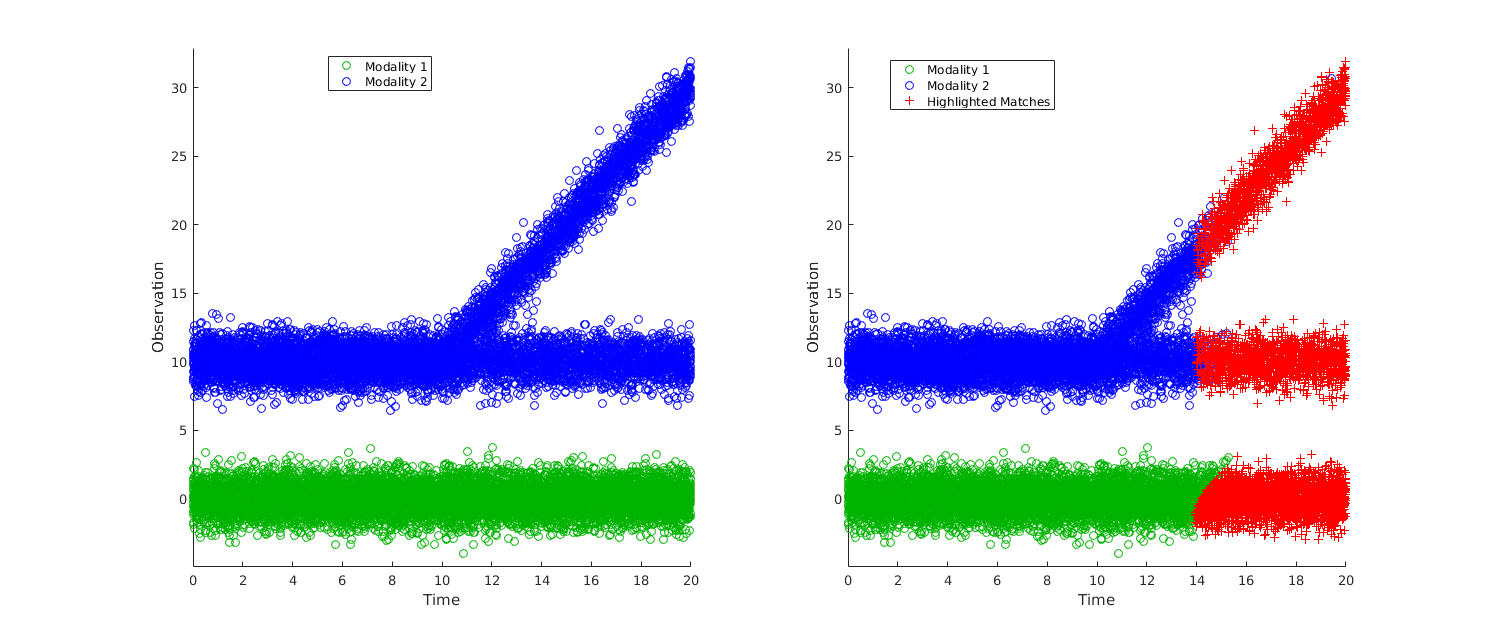
\includegraphics[width=\textwidth]{./FeatureComparison.png}
  \caption{Synthetic Dataset}
\end{figure}

\begin{figure}
  \centering
  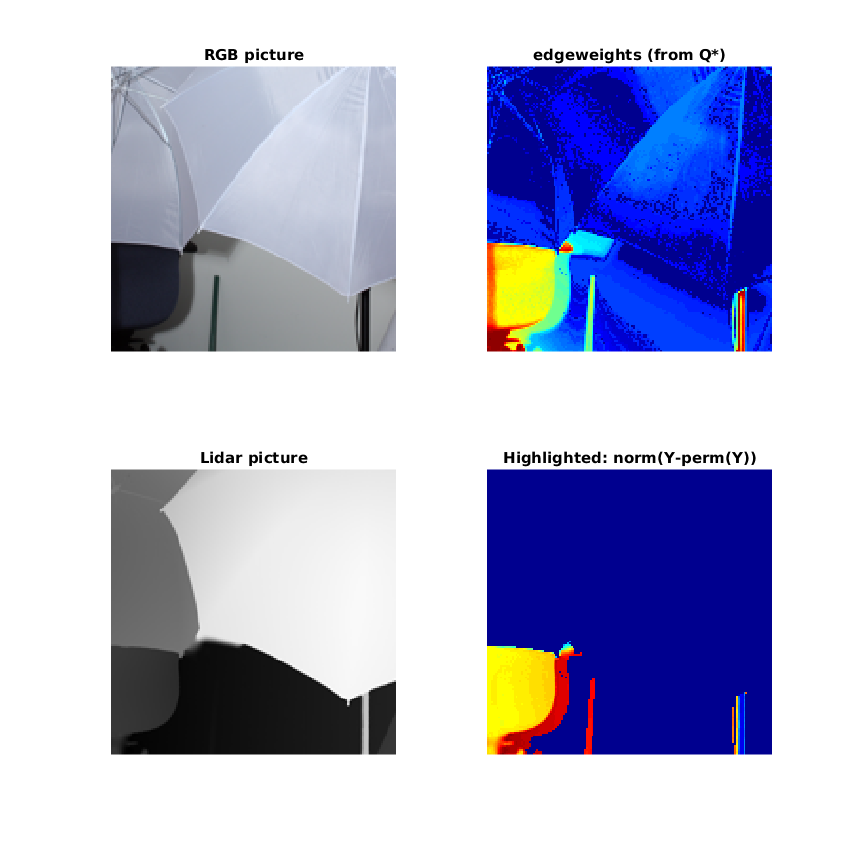
\includegraphics[width=\textwidth]{./UmbrellaFeatureComparison.png}
  \caption{Umbrella Dataset}
\end{figure}

\begin{figure}
  \centering
  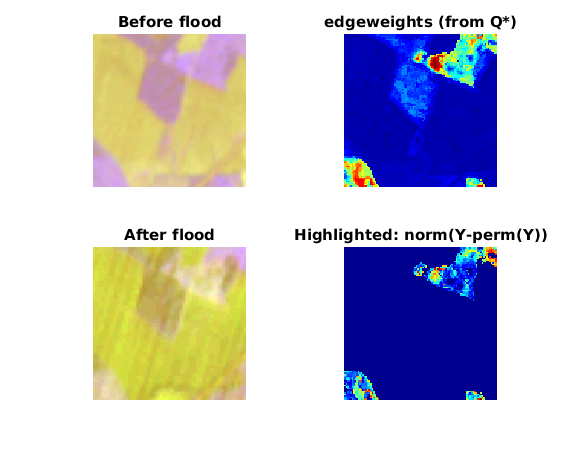
\includegraphics[width=\textwidth]{./FloodFeatureComparison.png}
  \caption{Flood Dataset}
\end{figure}

\end{document}
